\chapter{Combinação Linear}
\thispagestyle{empty}

\section{Introdução}
Já sabemos que  dados vetores $u$ e $v$ de um espaço vetorial $V$ sobre um corpo $\mathbb{K}$,  os vetores $u+v$ e  $\alpha u+\beta v$ estão   em $V$, quaisquer que sejam os escalares $\alpha$ e $\beta$. Nesta seção veremos que qualquer vetor $v \in V$ pode ser escrito como soma de  produtos por escalar de outros vetores de $V$.  \textbf{Atenção.} \textit{Estas notas de aulas tem como objetivo guiar os alunos nos  estudos da disciplina álgebra linear, nas turmas de minha responsabilidade, nos cursos de engenharia da UNIVASF. O uso das mesmas  não dispensa  a leitura  dos livros didáticos indicados nas referências bibliográficas da disciplina, bem como a resolução de exercícios propostos nos mesmos}.

\section{Combinação Linear}


\textbf{Definição.} Sejam $V$ um espaço vetorial sobre um corpo $\mathbb{K}$,  $v_1, v_2,..., v_n$ vetores de $V$.  Dizemos que o vetor $v \in V$ é uma \textit{ combinação linear} dos vetores $v_1, v_2,..., v_n$, se existem  escalares $a_1, a_2, ..., a_n \in \mathbb{K}$  tais que
\begin{equation}v=a_1v_1+a_2v_2+...+a_n v_n. \end{equation}

\vspace{0.3cm}

A Figura 1 ilustra uma combinação linear de vetores no plano.
\begin{centering}
\begin{figure}[h!]
%\centering
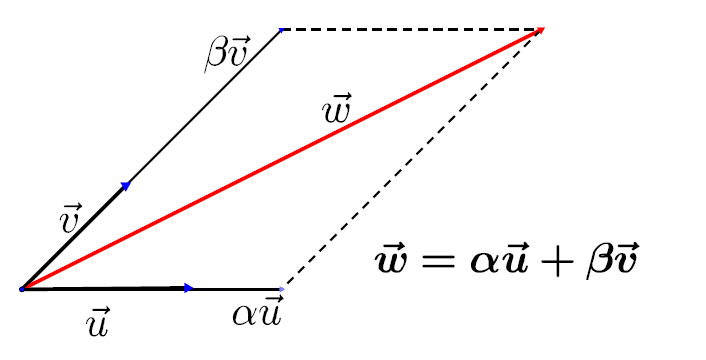
\includegraphics[width=1.0\textwidth]{chapters/combinacao_linear/img/com_linear}
\caption{\footnotesize{ O vetor $\vec{w}$ é uma combinação linear dos vetores $\vec{u}$  e $\vec{v}$}}
\label{fig:comb_linear}
\end{figure}
\end{centering}


\section{Exemplos}
\begin{enumerate}
\item  Considere o espaço vetorial  $\mathbb{P}_2$ dos polinômios de grau menor  ou igual a 2 sobre $\mathbb{R}$. O polinômio $p(x)=5x^2-3x-3$ é uma combinação linear dos polinômios $p_1(x)=x^2-x+1$ e $p_2(x)=-3x^2+x+5$. De fato, verifica-se que $p(x)=2p_1(x)-p_2(x)$.

\item Dados os vetores $v_1=(1,-3,2)$ e $v_2=(2,4,1)$ do espaço vetorial  $\mathbb{R}^3$, temos:
  \begin{enumerate}[label=(\alph*)]
\item O vetor $v=(-4,-18,1)$ é uma combinação linear dos vetores $v_1$ e $v_2$.
\item O vetor $w=(4,3,-6)$  não é uma combinação linear dos vetores $v_1$ e $v_2$.

De fato, no item (a) observe que $$v=2v_1+(-3)v_2.$$  Uma forma de obter os escalares $2$ e $-3$  é  usando a definição de combinação linear, de onde vem a seguinte equação
\begin{align*}(-4,-18,1)&=a_1(1,-3,2)+a_2(2,4,1)\\
                                    &=(a_1+2a_2, -3a_1+4a_2,2a_1+a_2).
\end{align*}

Da iguadade de vetores em $\mathbb{R}^3$, obtemos o sistema linear

\begin{align}
a_1+2a_2&=-4 \nonumber  \\
-3a_1+4a_2 &=-18\nonumber \\
2a_1+a_2&=1. \label{ex2a}
\end{align}
Resolvendo o sistema \eqref{ex2a}, concluimos que $a_1=2$ e $a_2=3$ formam a única solução do mesmo.

Já para o item (b), usamos o mesmo procedimento, obtemos o sistema linear
\begin{align} a_1+2a_2&=4 \nonumber  \\ -3a_1+4a_2 &=3\nonumber \\ 2a_1+a_2&=-6, \label{ex2b}\end{align}   o qual não possui solução. Logo, o vetor $ W$ não é uma combinação linear dos vetores $v_1$ e $v_2$.

\end{enumerate}

\item  O vetor $(3,4)$ do  $\mathbb{R}^2$ pode ser escrito de infinitas maneiras como combinação linear do vetores $(1,0)$, $(0,1)$ e $(2,-1)$. Com efeito, por  definição, o vetor  $(3,4)$ será uma combinação linear dos vetores $(1,0)$, $(0,1)$ e $(2,-1)$ se existirem  escalares $a_1$, $a_2$ e $a_3$ tais que $$(3,4)=a_1(1,0)+ a_2(0,1)+a_3(2,-1).$$ Resolvendo essa equação vetorial, obtemos $$(3,4)=(a_1+2a_3, a_2-a_3),$$  de onde vem   o sistema linear
\begin{align} a_1+2a_3&=3 \nonumber  \\ a_2-a_3&=4. \label{ex3a}\end{align}

Note que o sistema linear \eqref{ex3a} possui mais incógnitas do que equação. Logo  é um sistema indeterminado, ou seja, possui infinitas soluções. Considerando $a_3$ como uma variável livre, a solução geral o sistema linear \eqref{ex3a} é dada por $$\{ ( 3-2a_3, 4+a_3, a_3); a_3 \in \mathbb{R}\}.$$




\end{enumerate}



\section{Subespaços Gerados}

Sejam $V$ um espaço vetorial sobre um corpo  $\mathbb{K}$ e $W=\{v_1, v_2,..., v_n\}$ um subconjunto não vazio de $V$. O conjunto $S$ de \textbf{todas as combinações lineares} dos vetores de $W$ é um subespaço vetorial de $V$.

De fato, $S\neq \emptyset $ pois $$0=0v_1+0v_2+...+0v_n.$$  Isto é, o vetor nulo de $V$ pode ser escrito como uma combinação linear dos vetores de $W$. Agora,  suponha que $w_1$ e $w_2$ são vetores quaisquer de $S$, então existem escalares $a_1, a_2,...,a_n$ e $b_1, b_2,..,b_n$ tais que $$w_1=a_1v_1+ a_2v_2+...+a_nv_n \; \:\text{e} \; \;  w_2=b_1v_1+ b_2v_2+...+b_nv_n.$$ Daí, vem que $$ w_1+w_2=(a_1+b_1)v_1+ (a_2+b_2)v_2+...+(a_n+b_n)v_n .$$ Logo, $w_1+w_2 \in S$ pois também é uma combinação linear de vetores de $W$. Além disso, tem-se que $$\alpha \cdot w_1=(\alpha a_1)v_1+ (\alpha a_2)v_2+...+(\alpha a_n)v_n $$ e, dessa maneira, $\alpha \cdot w_1 \in S$, para todo escalar $\alpha$ e todo $w_1 \in S$. Portanto, $S$ é um subespaço vetorial de $V$.


\vspace{0.3cm}
\textbf{\textit{Observações.}}
  \begin{enumerate}%[label=(\alph*)]
\item Diz-se que $S$ é o  \textit{subespaço  gerado} pelos  vetores  $v_1, v_2,..., v_n$. Ou que $S$ é o  \textit{subespaço  gerado} por $W$. Denota-se $$S=G(W)=[v_1, v_2,..., v_n].$$

\item Os vetores  $v_1, v_2,..., v_n$ são chamados de vetores \textit{geradores}  do subespaço $S$, enquando $W$ é o conjunto \textit{gerador}  do subespaço $S$.

\item Define-se $G(\emptyset)=\{0\}$. Isto é, o espaço gerado pelo conjunto vazio é  o espaço vetorial formado apenas pelo vetor nulo.

\item $W \subset G(W)$. Ou seja, um conjunto de geradores  sempre está contido no subespaço gerado por ele.

\item Todo subconjunto $W $ de um espaço vetorial $V$ gera um subespaço de $V$, podendo $G(W)=V$. Neste caso, diz-se que  $W$ é um gerador de $V$.

\end{enumerate}

\section{Exemplos}

\begin{enumerate}
\item  Em $\mathbb{R}^2$ o vetor  $(1,1)$ gera o subespaço $$U= \{  (x,x); x \in \mathbb{R}\}.$$ Com efeito, qualquer vetor $(x,x) \in U$ pode ser escrito da seguinte maneira $$(x,x)=x\cdot (1,1).$$ Logo, $ U=[(1,1)]$.

\item Os vetores $(1,0)$ e $(0,1)$ geram o espaço $\mathbb{R}^2$. De fato, dado um  vetor $(x,y)$, qualquer, de $\mathbb{R}^2$, têm-se $$(x,y)=x \cdot(1,0)+ y\cdot (0,1).$$ Ou seja, qualquer vetor do $\mathbb{R}^2$ se escreve como uma combinação linear dos vetores $(1,0)$ e $(0,1)$. Portanto, $$[(1,0),(0,1)]=\mathbb{R}^2.$$

\item Um vetor $(x,y)$, qualquer, de $\mathbb{R}^2$, também pode ser escrito do seguinte modo: $$(x,y)=\dfrac{x+y}{2}(1,1)+ \dfrac{y-x}{2}(-1,1).$$ Ou seja, qualquer vetor do $\mathbb{R}^2$ também pode ser escrito como uma combinação linear dos vetores $(1,1)$ e $(-1,1)$. Portanto, $$[(1,1),(-1,1)]=\mathbb{R}^2.$$  \textbf{\textit{Observação.}} Os escalares $\dfrac{x+y}{2}$ e $\dfrac{y-x}{2}$ podem ser calculados resolvendo-se a equação $$(x,y)=a_1(1,1)+a_2(-1,1)$$ em função de $x$ e $y$.



\item O conjunto de polinômios $\{1, t, t^2\}$  gera todo o espaço  $\mathbb{P}_2$. De fato, qualquer polinômio $p(t)$ de grau igual ou menor do que 2 se escreve da seguinte maneira $p(t)=a_2t^2+a_1t+a_0$.

\item Em $\mathbb{M}(2,2)$, temos $\begin{bmatrix}a & b\\0 & c \end{bmatrix} = a\begin{bmatrix} 1 & 0 \\ 0 & 0\end{bmatrix}+b  \begin{bmatrix} 0 & 1\\ 0 & 0\end{bmatrix} + c \begin{bmatrix}0 & 0 \\ 0 & 1 \end{bmatrix}$. Logo, o subespaço das matrizes triângulares superiores de ordem 2 é gerado pelas matrizes $\begin{bmatrix} 1 & 0 \\ 0 & 0\end{bmatrix}$, $\begin{bmatrix} 0 & 1\\ 0 & 0\end{bmatrix}$ e $ \begin{bmatrix}0 & 0 \\ 0 & 1 \end{bmatrix}$.

\item  Se $[u_1,u_2,..,u_k]=U$ e $[w_1,w_2,...,w_k]=W$, então $U+W=[u_1,u_2,..,u_k, w_1,w_2,...,w_k]$. Isto é, se os vetores $u_1,u_2,..,u_k$ geram o subespaço vetorial $U$; e se os vetores $w_1,w_2,...,w_k$ geram o subespaço vetorial $W$, então o subespaço vetorial $U+W$ é gerado pela reunião dos vetores geradores de $U$ com os vetores geradores de $W$.

\end{enumerate}

\section{Dependência e Independência  Linear}

\textbf{Definição.} Sejam $V$ um espaço vetorial sobre um corpo  $\mathbb{K}$ e $v_1, v_2,..., v_n$ vetores de  $V$.  Dizemos que o conjunto $\{v_1, v_2,..., v_n\}$ é um conjunto \textit{linearmente independente (LI)}, ou que os vetores $v_1, v_2,..., v_n$  são $LI$, se a equação $$a_1v_1+a_2v_2+...+a_nv_n=0_v$$ admite apenas a solução nula.  Isto é, se $a_1=a_2=...=a_n=0$.

\vspace{0.3cm}

No caso em que exista algum $a_i \neq 0$ dizemos que o o conjunto $\{v_1, v_2,..., v_n\}$ é um conjunto \textit{linearmente dependente (LD)}, ou que os vetores $v_1, v_2,..., v_n$  são $LD$.

\vspace{0.3cm}

\textit{\textbf{Observação.}} O símbolo $0_v$ na definição acima indica o vetor nulo do espaço vetorial $V$ em questão.

\vspace{0.3cm}
O teorema a seguir estabelece outra caracterização da  depência linear.

\vspace{0.3cm}

 \textit{\textbf{Teorema 1.} O conjunto $\{v_1, v_2,..., v_n\}$ é $ LD$ se, e somente se, pelo menos um desses vetores for combinação linear dos demais.}

\vspace{0.3cm}

\textbf{\textit{Demonstração.}}

Suponha que $\{v_1, v_2,..., v_n\}$ é um conjunto $LD$.  Então, por definição,  a equação

\begin{equation*}
a_1v_1+a_2v_2+...+a_nv_n=0 \label{ld1}
\end{equation*}
admite uma solução diferente da trivial. Isto é, existe uma solução $( a_1, a_2,..., a_n) $ onde pelo menos um $a_i \neq 0$. Vamos supor, sem perda de generalidade, que $a_1 \neq 0$. Assim, obtemos
 \begin{align*}
a_1v_1+a_2v_2+...+a_nv_n&=0 ;\\
a_1v_1&=-a_2v_2-a_3v_3-...-a_nv_n ;\\
v_1&=\dfrac{1}{a_1}(-a_2v_2-...-a_nv_n);\\
v_1&=-\dfrac{a_2}{a_1}v_2-\dfrac{a_3}{a_1}v_3-...-\dfrac{a_n}{a_1}v_n.
\end{align*}
Logo, $v_1$ é uma combinação linear de $\{ v_2,..., v_n\}$.

Por outro lado, suponha que algum dos vetores de $\{v_1, v_2,..., v_n\}$ é uma combinação linear dos demais. sem perda de generalidade, vamos supor que $v_1$ seja esse vetor. Pela definição de combinação linear, existem escalares $( a_2, a_3, ..., a_n) $ tais que
 \begin{align*}
v_1= a_2v_2+a_3v_3+...+a_nv_n.
\end{align*}
Dessa equação, obtemos
 \begin{align*}
v_1-a_2v_2-a_3v_3-...-a_nv_n=0
\end{align*}
que é uma combinação linear nula tendo  o número 1 como o coeficiente de $v_1$. Logo, qualquer solução dessa equação será diferente da solução nula. Portanto, o conjunto de vetores $\{v_1, v_2,..., v_n\}$  é um conjunto $LD$. $\Box$

\vspace{0.3cm}

Equivalentemente ao \textbf{Teorema1} , temos o seguinte:


\vspace{0.3cm}

 \textit{\textbf{Teorema 2.}  O conjunto $\{v_1, v_2,..., v_n\}$ é LI se, e somente se, nenhum desses vetores for combinação linear dos demais.}

\section{Exemplos}
\begin{enumerate}
\item \textit{Em $\mathbb{R}^2$, os vetores $(1,1)$  e $(-1,1)$ são vetores LI. }

 De fato, sejam $a_1$ e $a_2$ tais que  \begin{align*} a_1(1,1) + a_2(-1,1)=(0,0)\\ (a_1-a_2, a_1+a_2)=(0,0).\end{align*} Daí, obtemos o sistema linear
\begin{align*} a_1-a_2&=0   \\ a_1+a_2 &=0\end{align*}    cuja solução é $a_1=a_2=0$.

\item \textit{Em $\mathbb{R}^2$, Os vetores $(1,0)$, $(0,1)$ e $(2,-1)$ são linearmente dependentes. }  De fato, note que o vetor $(2,-1)$ é uma combinação linear dos vetores $(1,0)$ e $(0,1)$  pois $$(2,-1)=2(1,0-1(0,1).$$  Logo pelo  Teorema 1,  o conjunto $\{(1,0), (0,1), (2,-1)\}$ é LD.



\item Sejam  $V$  um espaço vetorial sobre um corpo $\mathbb{K}$ e  vetores $u, v \in V$. Provar que se $u$ e $v$ são LI, então $u + v$ e $ u – v$ também o são.

\textbf{\textit{Demonstração.}} Como queremos mostrar que os vetores $u + v$ e $ u – v$ são LI, considere a combinação linear dando o vetor nulo $ a(u+v)+b(u-v)=0_v$. Devemos mostrar que $a=b=0$.

\begin{align*} a(u+v)+b(u-v)&=0_v   \\
                   au+av+bu-bv &=0_v\\
                   (a+b)u+(a-b)v&=0_v
\end{align*}
Como os vetores $u$ e $v$ são LI, por hipótese, segue da terceira equação que $a$ e $b$ deve satisfazer o sistema de equações
\begin{align*} a+b&=0   \\ a-b &=0,\end{align*} cuja solução é $a=b=0$. $\Box$


\item \textit{ Seja $V$ o espaço vetorial das funções reais contínuas. O conjunto $\{ e^x, e^{-x}\}$, onde $e$ é o número de Euler (base dos logaritmos naturais),  é LI.}

\textbf{\textit{Demonstração.}} Devemos mostrar que a equação $ae^x+ be^{-x}=0$ admite apenas a solução $a=b=0$.  Dada a equação

\begin{equation}
ae^x+ be^{-x}=0, \label{exp1}
\end{equation}
calculemos  a derivada das funções de  ambos os menbros. Daí,  obtemos
\begin{equation}
ae^x- be^{-x}=0.\label{exp2}
\end{equation}

Somando as equações \eqref{exp1} e \eqref{exp2}, vem que

\begin{equation*}
2ae^x=0.
\end{equation*}

Como $2e^x \neq 0$ para todo $x$ real, segue que $a=0$.  Substituindo  o valor de $a$ na equação \eqref{exp1}, obtemos
\begin{equation*}
be^{-x}=0.
\end{equation*}
Como $e^{-x}\neq 0$ para todo $x$ real, segue que $b=0$. Logo, $a=b=0$  e equação $ae^x+ be^{-x}=0$  admite apenas a solução nula. Portanto, o conjunto $\{ e^x, e^{-x}\}$
é LI como queríamos demosntrar. $\Box$
\end{enumerate}

\subsection{Propriedades da Dependência e Independência Linear}

Seja $V$ um espaço vetorial sobre um corpo $\mathbb{K}$.
\begin{enumerate}
\item Se  $W=\{w\}$ e $w \neq 0_v$, então $W$ é LI.
\item Se um conjunto $W \subset V$  contém o vetor nulo, então $W$ é LD.
\item 	Se uma parte do conjunto $W \subset V$  é LD, então $W$  é também LD.
\item 	Se um conjunto  $W$  é LI, qualquer parte $\bar{W}$ de $W$  também é  LI.
\item 	Se $\{v_1, v_2,..., v_n\}$  é LI e  $\{v_1, v_2,..., v_n, w\}$ é LD,então $w$ é combinação linear de  dos vetores  $v_1, v_2,..., v_n$.

\textbf{\textit{Demontração.}} Para provar (i), considere a equação $ \alpha w=0_v$. Como $w\neq 0_v$, então $\alpha=0$ é a única solução possível. Logo pela definição de dependência linear, $W$ é LI.

 Para provar (ii), suponha que  $W$ é um subconjunto de $V$ contendo o vetor nulo. Como podemos escrever o vetor nulo como combinação linear dos demais vetores (basta tomar os coeficientes da combinação linear como sendo o número zero), então pelo Teorema 1, $W$ é um conjunto LD.

Para mostrar que (iii) vale, seja $W=\{v_1, v_2,..., v_k, v_{k+1},...,v_n\}$ um conjunto de $V$ e seja $\bar{W}=\{v_1, v_2,..., v_k\} \subset W$ um conjunto  $LD$. Logo, existe pelo menos um vetor  de $\bar{W}$  que é uma combinação linear dos demais vetores de $\bar{W}$. Digamos que $v_1$ seja esse vetor. Logo,  existem escalares $a_2,...a_k$ tais que $v_1=a_2 v_2+...+ a_kv_k$. Como podemos escrever, $$v_1=a_2 v_2+...+ a_kv_k+0v_{k+1}+...+0v_n,$$
segue $v_1$ também é uma combinação linear dos demais  vetores de $W$ e, portanto, $W$ é um conjunto LD.



Os itens (iv) e (v) fica como exercício.$\Box$


\end{enumerate}


\section{Exercícios Propostos}


\begin{enumerate}

\item 	Sejam os vetores $u = (2,-3,2)$ e $v = (-1,2,4)$ em $\mathbb{R}^3$.
\begin{enumerate}[label=(\alph*)]
\item 	Escrever o vetor $w = (7,-11,2)$ como combinação linear de $u$ e $v$.
\item 	Para que valor de $k$ o vetor $( -8, 14, k)$ é combinação linear de $u$ e $v$?
\item 	Determinar uma condição entre $a$, $b$ e $c$ para que o vetor $(a,b,c)$ seja uma combinação linear de $u$ e $v$.
\end{enumerate}


\item	Consideremos no espaço $\mathbb{P}_2= {at^2 + bt + c; a, b,c \mathbb{R}}$ os vetores $p(t) = t^2 – 2t +1$,
      $q(t) = t + 2$ e $h(t)= 2t^2-t$.
\begin{enumerate}[label=(\alph*)]
\item	Escrever o vetor $m(t) = 5t^2 – 5t + 7$ como combinação linear de $p(t)$, $q(t)$ e $h(t)$.
\item	Escrever o vetor $m(t) = 5t^2 – 5t + 7$ como combinação linear de $p(t)$ e $q(t)$.
\item	Determinar uma condição para $a$, $b$ e $c$ de modo que o vetor $at^2 + bt + c$ seja combinação linear de
      $q(t)$ e $h(t)$.
\item	É possível escrever $p(t)$ como combinação linear de $q(t)$ e $h(t)$?
\end{enumerate}

\item	Considere o subespaço de $\mathbb{R}^4$:
 $$S = [(1,1,-2,4), (1,1,-1,2),(1,4,-4,8)]$$
\begin{enumerate}[label=(\alph*)]
\item	o vetor $(2/3, 1, -1, 2)$ pertence a $S$?
\item	o vetor $(0,0,1,1)$ pertence a $S$?
\end{enumerate}

\item Seja $W$ o subespaço de $\mathbb{M}(2,2)$ definido por $$\left\{ \begin{bmatrix}2a & a+2b \\ 0 & a-b \end{bmatrix}; a,b \in \mathbb{R} \right\}.$$
\begin{enumerate}[label=(\alph*)]
\item $ \begin{bmatrix}0 & -2 \\ 0 & 1 \end{bmatrix} \in W$?
\item  $ \begin{bmatrix}0 & 2 \\ 0 & 1 \end{bmatrix} \in W$?
\end{enumerate}


\item  Seja $W$ o subespaço de $\mathbb{M}(3,2)$  gerado pelas matrizes $\begin{bmatrix}0 & 0 \\ 1& 1 \\0 & 0 \end{bmatrix}$ , $ \begin{bmatrix}0 & 1 \\ 0& -1 \\1& 0 \end{bmatrix}$ e  $\begin{bmatrix}0 & 1\\ 0& 0\\ 0 & 0 \end{bmatrix}$. Verifique se a matriz $\begin{bmatrix}0 & 2\\ 1& 2\\ 3& 0 \end{bmatrix} \in W$.


\item Seja $V=\mathbb{C}[0,1]$ o espaço vetorial das funções reais contínuas no intervalo $[0,1]$. Verifique se cada um dos  subconjutnos a seguir são LI em $V$.

\begin{enumerate}[label=(\alph*)]
\item $\{ x, x+1, x^2-1\} $
\item $\{1, e^x, e^{-x}\}$
\item $\{ senx, cosx\}$.
\end{enumerate}

\item Dados vetores $v_1, v_2,..., v_n$  de um espaço vetorial $V$,  prove que se $w\in V$  é uma combinação linear dos vetores  $v_1, v_2,..., v_n$, então $$[v_1, v_2,..., v_n, w]=[v_1, v_2,..., v_n].$$

\item Sejam $v_1, v_2,..., v_n$ vetores linearmente independentes de um espaço vetorial $V$. Prove que  se $a_1v_1+a_2v_2+...+a_n v_n=b_1v_1+b_2v_2+...+b_n v_n$, então  $a_1=b_1$, $a_2=b_2$,..., $a_n=b_n$.
\item Sejam $V$ um espaço vetorial  e $ u, v, w \in V$. Prove que o conjunto $\{ u, v, w\}$ é LI se, e somente se, o conjunto $\{ u+v, u+w, v+w\} $ é LI.

\item Sejam $V$ um espaço vetorial  e $ u, v, w \in V$. Suponha que $\{ u, v, w\}$ é LI. Dado $t \in V$, existem escalares $\alpha$, $\beta$ e $\gamma$ tais que  $t=\alpha u+\beta v+\gamma w$. Prove que $\{u+t, v+t, w+t\}$ é LI se, e somente se, $\alpha+\beta+\gamma \neq 1$.

\end{enumerate}

%De acordo com a definição anterior, qualquer subespaço de  um espaço vetorial  $V$ deve, necessariamente, conter o vetor nulo de $V$. De fato, a operação de adição de vetores a ser considerada no subconjunto $W$ é  obrigatoriamente a mesma de $V$ e o elemento neutro dessa operação é único.
%
%\vspace{0.3cm}
%Todo espaço vetorial $V$ admite pelo menos dois subespaços: o conjunto formado apenas pelo vetor nulo  e o próprio espaço. Isto é,  $\{ 0\}$ e  $V$. Esses dois subespaços de $V$  são chamados de \textbf{subespaços triviais}.
%
%
%\vspace{0.3cm}
%
%Utilizar a definição de subespaço vetorial para  identificar se um subconjunto $W$  de um espaço vetorial $V$  é um subespaço é  uma atividade laboriosa, pois exige a verificação das oito propriedades,  (A1)-(A4) e (ME1)-(ME4), da definição de espaço vetorial. Felizmente, de acordo com a  próxima proposição,  não precisaremos fazer  a verificação de todas essas propriedades. De fato, sendo  $W$  um subconjunto de $V$,  as propriedades  das operações que são válidas em $V$ devem também ser válidas em $W$, desde que $W$ seja um conjunto fechado em relação a essas operações. Isto é, o resultado das operações realizadas com elementos de $W$  resultam em elementos de $W$.
%
% Um subespaço vetorial $W$ de um espaço vetorial $V$  fica caracterizado pela seguinte proposição:
%
%\textbf{Proposição.} Dados um espaço vetorial $V$ e  um subconjunto $W$ de $V$   não vazio. $W$ é um subespaço de  $V$ se as duas condições a seguir  forem satisfeitas:
%
%\begin{enumerate}[label=(\roman*)]
%\item Se $u$ e $v$ são vetores quaisquer de $W$, então $u+v \in W$;
%\item Se  $ \alpha \in \mathbb{R}$ e $ v$ é um vetor qualquer de $W$, então $\alpha v\in W$.
%
%\end{enumerate}
%
%\textbf{\textit{Observações.}}
%\begin{enumerate}%[label=(\roman*)]
%\item Todo subespaço $W$ de um espaço vetorial $V$ precisa, necessariamente, conter o vetor nulo de $V$. De fato, se tomarmos $\alpha=0$, por (ii),  temos $$0\cdot v=0 $$ para todo $v \in W$.
%
%\item Dessa forma,  se um subconjunto não vazio  $W$ de um espaço vetorial $V$ não possuir o vetor nulo de $V$,  então $W$ não pode ser um subespaço vetorial de $V$.
%\end{enumerate}
%
%\section{Exemplos}
%\begin{enumerate}
%
%
%\item Seja $V=\mathbb{R}^2=\{(x_1, x_2); x_i \in \mathbb{R}\}$ com as operações usuais de  soma de vetores e a multiplicação por escalar.  O subconjunto
%$$W=\{(x, y); y=kx, \; \text{$k$ é uma constante} \}$$ é um subespaço vetorial de $V$.
%
%\textbf{\textit{Demonstração.}}
%Observe que $W$ também pode ser escrito da seguinte maneira:
%$$W=\{(x, kx);  x \in \mathbb{R} \; \text{e}\; \text{$k$ constante} \}.$$   Primeiro é conveniente observar que $(0,0) \in W$. De fato, para $x=0$ teremos $kx=0$, para todo $k\in \mathbb{R}$. Logo, $(0,0) \in W$ e, desse modo, $W \neq \emptyset$.
%
%Agora sejam $u=(x_1, y_1)$ e $v=(x_2, y_2)$ vetores de $W$.  Dessa maneira, podemos escrever $u=(x_1, kx_1)$ e $v=(x_2, kx_2)$. Assim,
%\begin{align*}
%u+v &=(x_1, kx_1)+(x_2, kx_2)\\
%       &=(x_1+x_2, kx_1+kx_2)\\
%       &=(x_1+x_2, k(x_1+x_2)).
%\end{align*}
%Fazendo $x_3=x_1+x_2$, temos que $u+v =(x_3, kx_3)$. Logo, $u+v \in W$ e o item (i) é satisfeito.  Agora seja  $\alpha \in \mathbb{R}$ e $u=(x_1, y_1) \in W$. Assim
%\begin{align*}
%\alpha u &=\alpha(x_1,x_2)\\
%            &=\alpha (x_1, kx_1) \; \text{pois} \;  u \in W;\\
%       &=(\alpha x_1, \alpha k x_1).
%\end{align*}
% Fazendo $x_4=\alpha x_1$ temos que $\alpha u=(x_4, kx_4)$. Logo, $\alpha u \in W$ e o intem (ii) da proposição está satisfeito.  Poranto, $W$ é um subespaço vetorial de $V$. Observe ainda que os elementos de  $W$ descrevem uma reta passando pela origem.
%
%\item Seja $V=\mathbb{R}^2$ e $U=\{(x, 5x+3);  x \in \mathbb{R}\}$.  O subconjunto $U$ não é,  com as operações usuais de  soma de vetores e a multiplicação por escalar, um subespaço vetorial de $\mathbb{R}^2$.   De fato,  o vetor $\{(0,0\}$ não pertence a $W$. Observe que os elementos de $U$ descrevem uma reta em $\mathbb{R}^2$ que não passa pela origem.
%
%
%\item Todos os subespaços de $\mathbb{R}^2$ são:  $\{(0,0)\}$, o  $\mathbb{R}^2$  e os seus subconjuntos que descrevem  retas passando pela origem.
%
%\item Seja $W=\{(x,y,z) \in \mathbb{R}^3; ax+by+cz=0\}$.  Observe que $W$ descreve, em $\mathbb{R}^3$, um \textbf{plano que passa pela origem}.  $W$ é um subespaço vetorial de $\mathbb{R}^3$.
%
%\textbf{\textit{Demonstração.}}
%  Primeiro é conveniente observar que $(0,0,0) \in W$. De fato, para $x=y=z=0$ teremos $ax+by+cz=0$, quaisquer que sejam os escalares  $a,b,c \in \mathbb{R}$. Logo, $(0,0,0) \in W$ e, desse modo, $W \neq \emptyset$.
%
%Agora sejam $u=(x_1, y_1, z_1)$ e $v=(x_2, y_2, z_2)$ vetores de $W$.  Dessa maneira,  temos que $ax_1+bx_1+cz_1=0$ e  $ax_2+bx_2+c_z2=0$. Assim,  temos
%\begin{align*}
%u+v &=(x_1, y_1, z_1)+(x_2, y_2, z_2)\\
%       &=(x_1+x_2, y_1+y_2, z_1+z_2).
%\end{align*}
%Fazendo $x_3=x_1+x_2$,$y_3=y_1+y_2$ e $z_3=z_1+z_2$ temos que
%\begin{align*}
%ax_3+by_3+cz_3&=a(x_1+x_2)+b(y_1+y_2)+c(z_1+z_2)\\
%                             &=\underbrace{ax_1+by_1+cz_1}_{0}+\underbrace{ax_2+by_2+cz_2}_{0}\\
%                             &=0+0=0.
%\end{align*}
%Logo, $u+v  \in W$ e o item (i) é satisfeito.  Agora seja  $\alpha \in \mathbb{R}$ e $u=(x_1, y_1, z_1) \in W$. Assim, $ax_1+bx_1+cz_1=0$.
%\begin{align*}
%\alpha u &=\alpha(x_1,y_1, z_1)\\
%            &=\alpha (x_1,y_1, z_1) \\
%       &=(\alpha x_1, \alpha y_1, \alpha z_1).
%\end{align*}
% Fazendo $x_4=\alpha x_1$, $y_4=\alpha y_1$ e  $z_4=\alpha z_1$ temos que
%\begin{align*}
%ax_4+by_4+cz_4&=a(\alpha x_1)+b(\alpha y_1)+c(\alpha z_1)\\
%                              &=\alpha ( ax_1 +b y_1+cz_1)\\
%                             &=\alpha\underbrace{ax_1+by_1+cz_1}_{0}\\
%                             &=\alpha \cdot 0=0.
%\end{align*}
%Logo, $\alpha u \in W$ e o intem (ii) da proposição está satisfeito.  Portanto, $W$ é um subespaço vetorial de $\mathbb{R}^3$.
%
%
%\item Todos os subespaços de $\mathbb{R}^3$ são:  $\{(0,0,0)\}$, o  $\mathbb{R}^3$, os seus subconjuntos que descrevem  retas passando pela origem e os subconjuntos que descrevem planos passando pela origem.
%
%
%\item Considere em $\mathbb{M}(n,n)$  o conjunto $S$ das matrizes simétricas de ordem $n$.  $S$ é um subespaço vetorial de $\mathbb{M}(n,n)$ . Isto é, $$S=\{ A \in \mathbb{M}(n,n); A^T=A\}.$$ $S$ é um subespaço vetorial de $\mathbb{M}(n,n)$ .
%
%\textbf{\textit{Demonstração.}}
%Primeiro observe que a matriz nula de ordem $n$ é uma matriz simétrica. Logo, $ S \neq \emptyset$.  Agora sejam $A$ e $B$ matrizes simétricas de ordem $n$. Pela propriedade das matrizes  simétricas, temos que $$ (A+B)^T=A^T+B^T. $$
%Por outro lado, $A$ e $B$ são matrizes simétricas. Logo, $A^T=A$ e $B^T=B$. Daí, vem que  $$ (A+B)^T=A^T+B^T = A +B .$$ Ou seja, $A+B$ é uma matriz simétrica. Logo, $A+B \in  \mathbb{M}(n,n)$.
%
%Dado $\alpha \in \mathbb{R}$ e $A$ uma matriz simétrica de ordem $n$, temos, pela propriedade de matriz simétrica, que  $$(\alpha A)^T= \alpha A^T=\alpha A.$$ Assim, $\alpha A$ é uma matriz simétrica, ou seja, $\alpha A \in \mathbb{M}(n,n)$. Portanto, $S$ é um subespaço vetorial de $\mathbb{M}(n,n)$.
%
%
%\item Considere o sistema linear homogêneo $$AX=0$$ onde  $A$, a matriz dos coeficientes, tem  ordem $m \times n$, $X$ é a matriz das incógnitas  e tem ordem $n \times 1$ e $0$ pé matriz dos termos independentes e tem ordem $ m \times 1$.  Seja $S_h$ o conjunto das soluções desse sistema linear homogêo.  Isto é,
%$$S_h=\{ X \in \mathbb{M}(n,1); AX=0 \}.$$  $S_h$ é um subespaço vetorial de $\mathbb{M}(n,n)$ .
%\end{enumerate}
%
%\subsection{Intersecção de Subespaços}
%Seja  $V$ um espaço vetorial sobre um corpo $\mathbb{K}$. Suponha que $U$ e $W$ são  subespaços vetoriais de $V$. Então o conjunto
%$$U\cap W=\{ v \in V;  \; v \in U \; \text{e} \; v \in W \} $$ é um subespaço vetorial de $V$.
%
%\textbf{\textit{Demonstração.}}
%
%Primeiro note que $U\cap W \neq \emptyset$. Isto é, $0 \in U\cap W$. De fato,  como $U$ e $W$ são subespaços de $V$, então $0 \in U$ e $0 \in W$, logo $0 \in U\cap W$.
%
%Agora, vamos mostrar que a soma de dois vetores quaisquer de $U \cap W$ é um vetor de  $U \cap W$.  Para isso suponha que $u,v \in U\cap W$. Dessa forma temos:
%\begin{align*}
%u\in U\cap W&, \; \text{ logo $u \in U$ e $u \in W$};\\
%v\in U\cap W &, \; \text{logo  $v \in U$ e $v \in W$}.
%\end{align*}
%Dessa maneira, temos  $u, v \in U$;   e $u,v \in W$. Como $U$ e $W$ são subespaços, então $u+ v \in U$  e $u+v \in W$. Logo, $$u+ v \in U \cap W. $$
%
%Para mostrarmos que a multiplicação de um vetor de $U\cap W$ por um escalar  também é um vetor $U\cap W$,  considere $\alpha \in \mathbb{K}$  e $u \in U\cap W$.  Desse modo,  $u\in U$ e $u \in W$  (ambos são subespaços de $V$), então   $\alpha \cdot  u \in U$ e $\alpha \cdot  u \in W$.
%Logo, $\alpha \cdot  u\in U\cap W$. Dessa forma concluimos que $U\cap W$ é um subespaço vetorial de $V$.
%
%\subsubsection{Exemplos}
%\begin{enumerate}
%\item Considere os subespaços de $\mathbb{R}^3$
%$$ U= \{(x,y,z) \in \mathbb{R}^3 ; z=0\} $$ e  $$ W= \{(x,y,z) \in \mathbb{R}^3 ; x=0\}.  $$ Seja $(a, b, c)$ um vetor qualquer de $\mathbb{R}^3$. Observe que  $(a, b,c ) \in U\cap W$ se, e somente se,  $(a, b, c) \in U$ e $(a, b, c) \in W$, simultaneamente. Mas, isso somente ocorre se tivermos  $a=0$   e $c=0$. Logo, um  vetor $v$ do $\mathbb{R}^3$ está em $U \cap W$ se, e somente se, $v$ é do tipo $(0, b, 0)$. Assim, escrevemos $$U \cap W=\{(x, y, z) \in\mathbb{R}^3; x=z=0 \}=\{ (0,y,0); y \in \mathbb{R}\}.$$
%
%
%\item Considere em $\mathbb{R}^2$ os subespaços
%$$ U= \{(x,y) \in \mathbb{R}^2 ; y=x\} $$ e  $$ W= \{(x,y) \in \mathbb{R}^2 ; y=-x\}.  $$ Seja $(a, b)$ um vetor qualquer de $\mathbb{R}^2$. Observe que  $(a, b ) \in U\cap W$ se, e somente se,  $(a, b) \in U$ e $(a, b) \in W$, simultaneamente. Mas, isso ocorre somente  se tivermos  $b=a$   e $b=-a$. De onde concluímos que $b=0$ e $a=0$.  Logo, um  vetor $v$ do $\mathbb{R}^2$ está em $U \cap W$ se, e somente se, $v=(0, 0)$. Assim, obtemos $$U \cap W=\{(0,0) \}.$$
%
%\item  Sejam $V= \mathbb{M}(n,n)$ seja o espaço vetorial  das matrizes quadradas, com entradas reais,  de ordem $n$; $U$ o subconjunto  das matrizes triangulares inferiores e $W$ o subconjunto das matrizes triangulares superiores de ordem $n$.  É possível mostrar que $U$ e $W$ são subespaços vetoriais de $V$ (Exercício).  Observe que $U \cap W$ é o conjunto de todas as matrizes diagonais de ordem $n$.
%\end{enumerate}
%
%
%
%\subsection{Soma de Subespaços}
%Seja  $V$ um espaço vetorial sobre um corpo $\mathbb{K}$. Suponha que $U$ e $W$ são  subespaços vetoriais de $V$. Então o conjunto
%$$U+W=\{ v \in V; v=v_1+v_2, \; v_1 \in U \; \text{e} \; v_2 \in W \} $$ é um subespaço vetorial de $V$. O subespaço $U+W$ chama-se \textit{ soma} de $U$ e $W$.
%
%\textbf{\textit{Demonstração.}}
%
%Primeiro note que $U+W \neq \emptyset$. Isto é, $0 \in U+W$. De fato,  como $U$ e $W$ são subespaços de $V$, $0 \in U$ e $0 \in W$. Desse modo, como  $$0=0+0,$$ temos que $0$ pode ser escrito como a soma de um elemento de $U$ com um elemento de $W$.
%
%Sejam $u,v \in U+W$. Dessa forma podemos escrever
%\begin{align*}
%u&=u_1+w_1, \; \text{com $u_1 \in U$ e $w_1 \in W$};\\
%v&=u_2+w_2, \; \text{com $u_2\in U$ e $w_2 \in W$}.
%\end{align*}
%Assim, como $u_1, u_2 \in U$ (e $U$ é um subespaço de $V$), então $u_1+u_2 \in U$.  Do mesmo modo, como $w_1, w_2 \in W$ (e $W$ é um subespaço de $V$), então $w_1+w_2 \in W$.
%
%Desse modo,
%\begin{align*}
%u+v&=(u_1+w_1) + (u_2+w_2) \\
%         &=(u_1+u_2)+(w_1+w_2).
%\end{align*}
%Fazendo $u_3=u_1+u_2$ e $w_3=w_1+w_2$, temos que $u+v=u_3+w_3$, onde $u_3 \in U$ e $w_3 \in W$. Logo, $u+v \in U+W$.
%
%Agora, sejam $\alpha \in \mathbb{K}$  e $u \in U+W$.  Logo, existem $u_1 \in U$ e $w_1 \in W$ tais que $u=u_1+w_1$. Daí,
%\begin{align*}
%\alpha \cdot  u&=\alpha \cdot (u_1+w_1) \\
%         &=\alpha \cdot  u_1+\alpha \cdot  w_1.
%\end{align*}
%Note que $\alpha \cdot  u_1 \in U$ e $\alpha \cdot  w_1 \in W$, pois $U$ e $W$ sao subespaços.  Assim, fazendo $u_4=\alpha \cdot  u_1$ e $w_4=\alpha \cdot  w_1$, temos que $\alpha \cdot  u=u_4+w_4$, onde $u_4 \in U$ e $w_4 \in W$. Logo, $\alpha \cdot  u\in U+W$. Dessa forma concluimos que $U+W$ é um subespaço vetorial de $V$.
%
%\subsubsection{Exemplos}
%\begin{enumerate}
%\item Considere em  $\mathbb{R}^3$, os subespaços
%$$ U= \{(x,y,z) \in \mathbb{R}^3 ; z=0\} $$ e  $$ W= \{(x,y,z) \in \mathbb{R}^3 ; x=y=0\}.  $$ Dado   $(a, b, c)$ um vetor qualquer de $\mathbb{R}^3$, podemos escrever
%$$(a, b, c)= (a,b,0)+(0,0,c).$$
%
% Observe que  $(a, b,0 ) \in U$ e  $(0, 0, c) \in W$. Logo, $(a,b,c) \in U+W$.  Como $(a,b,c)$ é um vetor arbitrário de $\mathbb{R}^3$, concluimos que $$U+W=\mathbb{R}^3.$$
%
%
%\item Considere em $\mathbb{R}^2$, os subespaços
%$$ U= \{(x,y) \in \mathbb{R}^2 ; y=x\} $$ e  $$ W= \{(x,y) \in \mathbb{R}^2 ; y=-x\}.  $$ Seja $(a, b)$ um vetor qualquer de $\mathbb{R}^2$.  Note que  podemos escrever
%$(a, b)$ do seguinte modo: $$(a,b)=\left(\dfrac{a+b}{2},\dfrac{a+b}{2}   \right)+\left(\dfrac{a-b}{2},\dfrac{-a+b}{2}   \right).$$
%
%Como $\left(\dfrac{a+b}{2},\dfrac{a+b}{2}   \right) \in U$ e $\left(\dfrac{a-b}{2},\dfrac{-a+b}{2}   \right) \in W$, então $(a,b) \in U+W$.  Mas, $(a,b)$ é um vetor arbitrário de $\mathbb{R}^2$, logo $$\mathbb{R}^2 = U+W.$$
%
%
%
%\item  Sejam $V= \mathbb{M}(2,2)$ seja o espaço vetorial  das matrizes quadradas, com entradas reais,  de ordem $2$; $U$ o subconjunto  das matrizes triangulares inferiores e $W$ o subconjunto das matrizes triangulares superiores de ordem $2$. Dada  uma matriz  quadrada de ordem 2  qualquer, digamos, $\begin{bmatrix} a & b \\ c & d\end{bmatrix}$, podemos escrever
%$$\begin{bmatrix} a & b \\ c & d\end{bmatrix}= \begin{bmatrix} \frac{a}{2} & 0\\ c & \frac{d}{2}\end{bmatrix}+ \begin{bmatrix} \frac{a}{2} & b \\ 0 & \frac{d}{2}\end{bmatrix}.$$
%Ou seja, qualquer matriz quadrada de ordem 2 pode ser escrita como a soma de um elemento de $U$ (matriz triangular superior) e um elemento de $W$ ( matriz triangular superior). Portanto, $$ U+W=\mathbb{M}(2,2).$$
%
%\end{enumerate}
%
%
%
%
%\subsection{Soma direta}
%
%\textbf{Definição.}  Seja  $V$ um espaço vetorial. Suponha que $U$ e $W$ são  subespaços vetoriais de $V$.  Diz-se que $V$ é a \textit{soma direta } de $U$ e $W$, denota-se $V=U\oplus W$, se
%\begin{enumerate}[label=(\roman*)]
%\item $U \cap W =\{0\}$;
%\item $V=U+W$.
%\end{enumerate}
%
%\subsubsection{Exemplos}
%\begin{enumerate}
%\item No exemplo 1 ( Soma de Subespaços) os subespaços  $$ U= \{(x,y,z) \in \mathbb{R}^3 ; z=0\} $$ e  $$ W= \{(x,y,z) \in \mathbb{R}^3 ; x=y=0\}$$  são tais que  $\mathbb{R}^3=U+W$. Além disso, $U \cap W =\{ (0,0,0) \}$ ( verifique!). Portanto, $$ \mathbb{R}^3 =U\oplus W.$$
%
%\item  No exemplo 2 ( Soma de Subespaços) os subespaços $$ U= \{(x,y) \in \mathbb{R}^2 ; y=x\} $$ e  $$ W= \{(x,y) \in \mathbb{R}^2 ; y=-x\}$$ são tais que
%$\mathbb{R}^2 = U+W$. Além disso, Além disso, $U \cap W =\{ (0,0) \}$ ( verifique!). Portanto, $$ \mathbb{R}^2 =U\oplus W.$$
%
%\item O exemplo 3  (Soma de Subespaços)  temos $ U+W=\mathbb{M}(2,2)$, mas essa soma não pode ser uma soma direta por que $U \cap W $ é formado por todas as matrizes diagonais de ordem 2.
%
%\end{enumerate}
%
%
%
%
%
%
%\section{ Exercícios}
%
%
%\begin{enumerate}
%
%\item  Mostre que $W=\{ ( x, y, z) \in \mathbb{R}^3; z-y=0 \}$ é um  subespaço  vetorial de $\mathbb{R}^3$.
%
%\item Seja $S=\{ (x,y,z) \in \mathbb{R}^3; x+y+z=0\}$  um  plano do $\mathbb{R}^3$  passando pela origem. Mostre que $S$ é um subespaço vetorial  de $\mathbb{R}^3$.
%
%
%\item  Mostre que cada um dos subconjuntos de $\mathbb{R}^4$ a seguir são subespaços vetoriais.
%
%\begin{enumerate}[label=(\alph*)]
%\item $W_1=\{ ( x, y, z, t) \in \mathbb{R}^4; x+y=0 e z-t = 0\}$
%\item $W_2=\{ ( x, y, z, t) \in \mathbb{R}^4; 2x+y-t=0 e z = 0\}$
%\end{enumerate}
%
%\item Verifique se os subconjuntos $U$ e $W$, abaixo, são subespaços vetoriais de $\mathbb{M}(2,2)$.
%\begin{enumerate}[label=(\alph*)]
%\item $U=\left\{ \begin{bmatrix}  a & b\\ c & d \end{bmatrix}; b=c \; \text{e} \; a,b,c,d \in \mathbb{R}\right\}$
%\item $W=\left\{ \begin{bmatrix}  a & b\\ c & d \end{bmatrix}; b=c+1 \; \text{e} \; a,b,c,d \in \mathbb{R}\right\}$
%\end{enumerate}
%
%\item Considere os  subconjuntos de $\mathbb{R}^3$: $U=\{(x, x, x); x \in \mathbb{R} \}$  e $W=\{(x, y, 0); x, y \in \mathbb{R} \}$.
%\begin{enumerate}[label=(\alph*)]
%\item Mostre que $U$ é um subespaço vetorial   de $\mathbb{R}^3$;
%\item Mostre que $W$ é um subespaço vetorial   de $\mathbb{R}^3$;
%\item Mostre que $\mathbb{R}^3= U \oplus W$.
%\end{enumerate}
%
%\item Mostre que o subcojunto das matrizes anti-simétricas de ordem $n$  é um subespaço vetorial de  $\mathbb{M}(n,n)$.
%
%\item Seja $V=\mathbb{F}(\mathbb{R}, \mathbb{R})$ o espaço vetorial  de todas as funções reais e $$P=\{f \in V; f(-x)=f(x), \forall  x \in \mathbb{R} \}. $$ Ou seja, $P$ é o subconjunto das funções pares. Mostre que $P$ é um subespaço vetorial de $V$.
%
%\item Seja $V=\mathbb{F}(\mathbb{R}, \mathbb{R})$ o espaço vetorial  de todas as funções reais.  Verifique se os seguintes subconjuntos de $V$ são subespaços vetoriais.
%\begin{enumerate}[label=(\alph*)]
%\item $W_1 = \{ f \in V; f \; \text{ é contínua}\}$
%\item $W_2 = \{ f \in V; f \; \text{ é derivável}\}$
%\item $W_3 = \{ f \in V; f \; \text{ é integrável}\}$
%\end{enumerate}
%
%item  Sejam $U= \left\{ \left[\begin{array}{cc} a& b\\ c& d\end{array}\right] \in \mathcal{M}(2,2); \; b=c\right\}$ e $W= \left\{ \left[\begin{array}{cc} a& b\\ c& d\end{array}\right] \in \mathcal{M}(2,2); \; a=d=0\; {e} \; b=-c\right\}$.
%    \begin{enumerate}
%    \item Mostre que $U$ e $V$ são subespaços vetoriais de $ \mathcal{M}(2,2)$.
%    \item Mostre que $ \mathcal{M}(2,2)=U \bigoplus V$.
%    \end{enumerate}
%
%
%
%\end{enumerate}
